\documentclass[dvipdfmx]{jsarticle}


\usepackage{tcolorbox}
\usepackage{color}
\usepackage{listings, plistings}

%% ノート/latexメモ
%% http://pepper.is.sci.toho-u.ac.jp/pepper/index.php?%A5%CE%A1%BC%A5%C8%2Flatex%A5%E1%A5%E2

%% JavaScriptの設定
%% https://e8l.hatenablog.com/entry/2015/11/29/232800
\lstdefinelanguage{javascript}{
  morekeywords = [1]{ %keywords
    await, break, case, catch, class, const, continue, debugger, default, delete, 
    do, else, enum, export, extends, finally, for, function, function*, if, implements, import, in, 
    instanceof, interface, let, new, package, private, protected, public, return, static, super,
    switch, this, throw, try, typeof, var, void, while, with, yield, yield*
  },
  morekeywords = [2]{ %literal
    false, Infinity, NaN, null, true, undefined
  },
  morekeywords = [3] { %Classes
    Array, ArrayBuffer, Boolean, DataView, Date, Error, EvalError, Float32Array, Float64Array,
    Function, Generator, GeneratorFunction, Int16Array, Int32Array, Int8Array, InternalError,
    JSON, Map, Math, Number, Object, Promise, Proxy, RangeError, ReferenceError, Reflect,
    RegExp, Set, String, Symbol, SyntaxError, TypeError, URIError, Uint16Array, Uint32Array,
    Uint8Array, Uint8ClampedArray, WeakMap, WeakSet
  },
  morecomment = [l]{//},
  morecomment = [s]{/*}{*/},
  morestring = [b]{"},
  morestring = [b]{'},
  alsodigit = {-},
  sensitive = true
}

%% 修正時刻: Tue 2022/03/15 10:04:41


% Java
\lstset{% 
  frame=single,
  backgroundcolor={\color[gray]{.9}},
  stringstyle={\ttfamily \color[rgb]{0,0,1}},
  commentstyle={\itshape \color[cmyk]{1,0,1,0}},
  identifierstyle={\ttfamily}, 
  keywordstyle={\ttfamily \color[cmyk]{0,1,0,0}},
  basicstyle={\ttfamily},
  breaklines=true,
  xleftmargin=0zw,
  xrightmargin=0zw,
  framerule=.2pt,
  columns=[l]{fullflexible},
  numbers=left,
  stepnumber=1,
  numberstyle={\scriptsize},
  numbersep=1em,
  language={Java},
  lineskip=-0.5zw,
  morecomment={[s][{\color[cmyk]{1,0,0,0}}]{/**}{*/}},
  keepspaces=true,         % 空白の連続をそのままで
  showstringspaces=false,  % 空白字をOFF
}
%\usepackage[dvipdfmx]{graphicx}
\usepackage{url}
\usepackage[dvipdfmx]{hyperref}
\usepackage{amsmath, amssymb}
\usepackage{itembkbx}
\usepackage{eclbkbox}	% required for `\breakbox' (yatex added)
\usepackage{enumerate}
\usepackage[default]{cantarell}
\usepackage[T1]{fontenc}
\fboxrule=0.5pt
\parindent=1em
\definecolor{mygrey}{rgb}{0.97, 0.97, 0.97}

\makeatletter
\def\verbatim@font{\normalfont
\let\do\do@noligs
\verbatim@nolig@list}
\makeatother

\begin{document}

%\anaumeと入力すると穴埋め解答欄が作れるようにしてる。\anaumesmallで小さめの穴埋めになる。
\newcounter{mycounter} % カウンターを作る
\setcounter{mycounter}{0} % カウンターを初期化
\newcommand{\anaume}[1][]{\refstepcounter{mycounter}{#1}{\boxed{\phantom{aa}\textnormal{\themycounter}\phantom{aa}}}} %穴埋め問題の空欄作ってる。
\newcommand{\anaumesmall}[1][]{\refstepcounter{mycounter}{#1}{\boxed{\tiny{\phantom{a}\themycounter \phantom{a}}}}}%小さい版作ってる。色々改造できる。

%% 修正時刻: Tue 2022/03/15 10:04:411


\section{データベースを設計する}

\subsection{扱うデータ}

以下のようなデータを扱うこととする。

\vspace{3mm}
 \begin{tabular}{|c|} \hline
  菅原文太 \\
  40歳 \\
  1933年生まれ \\
  総務部 \\ \hline
 \end{tabular}
 \quad
 \begin{tabular}{|c|} \hline
  千葉真一 \\
  34歳 \\
  1939年生まれ \\
  営業部 \\ \hline
 \end{tabular}
 \quad
 \begin{tabular}{|c|} \hline
  北大路欣也 \\
  30歳 \\
  1943年生まれ \\
  経理部 \\ \hline
 \end{tabular}
 \quad
 \begin{tabular}{|c|} \hline
  梶芽衣子 \\
  26歳 \\
  1947年生まれ \\
  営業部 \\ \hline
 \end{tabular}
\vspace{3mm}

あなたがプログラマで、上のような社員名簿アプリを作成することになったとする。
PHP か Java でアプリを作成することになる。クライアントの会社の総務部がこの
アプリを使うことになる。そのアプリには社員の登録画面、一覧画面、編集画面、
削除画面などがあるだろう。そういった画面と処理をあなたは作らなければならない。

そのときに、データを保存するしくみとして、データベースを使うことになる。
かりに PHP でプログラミングするならば、PHPという言語を使って
データベースを操作することになる。

\subsection{primary key}

データベースにデータを格納する際には、そのデータに primary key (独自キー) が必要となる。
primary key とは、そのデータを他と区別するためのデータである。
菅原文太というデータは、この4つの中では独自であるが、他のデータを追加する際に、同じデータに出会う可能性
(同姓同名)を排除できない。
さらに日本語である以上、文字コードの問題を避けることもできない。つまり、同じ菅原文太という文字でも
UTF-8 と Shift\_JIS では別物と判定されるのである。

となると、この4つのデータには primary key となるものがないということになる。

このような場合、データベースの設計者が primary key を追加することになる。
ここでは 数字を primary key として追加する。
つまり、菅原文太は 1、千葉真一は 2 というふうにする。

\subsection{表を分ける}

4つの各データには、総務部、営業部、経理部 という部署名がはいっている。
これらは、部署データとして、別の表で管理するのが自然である。
そして、各人のデータから部署データを参照しているというふうにするのがよい。

\vspace{3mm}
XX会社 部署一覧 \\
\hspace{5mm}
\begin{tabular}{|c|} \hline
 総務部 \\
 営業部 \\
 経理部 \\
 開発部 \\ \hline
\end{tabular}\vspace{3mm}


\newpage
\section{データベースを作成する}

\subsection{ユーザーを作成して、データベースを作成する}

\subsubsection{MySQLの起動}

まず、MySQLを起動しなくてはならない。
\begin{enumerate}
 \item XAMPP コントロールパネルを管理者として起動する。
 \item MySQL の行の Start ボタンをクリックして MySQLを起動する。
\end{enumerate}

\vspace{3mm}
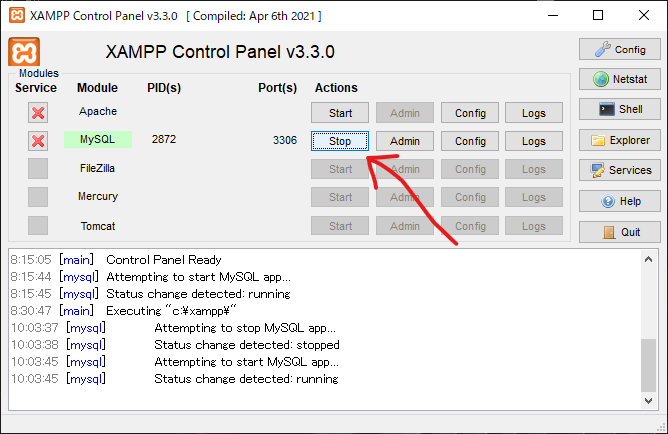
\includegraphics[width=10cm]{../06-mysql/02-mysql-start.png}
\vspace{3mm}


\subsubsection{rootユーザーでログインする}

データベースを作成するために、まずそのデータベースを扱うことのできるユーザーを作成する。

ユーザーを作成するために、まず管理者(root) でログインする。
MariaDBの場合、以下の手順でログインできる。

コマンドプロンプトを起動して、以下のコマンドを入力する。

\begin{tcolorbox}
 $>$ mysql -u root -p (Enterキー)\\
 $>$ Enter password: (何も入力せず、Enterキー)
\end{tcolorbox}

これで、4行ほどのメッセージと、次のプロンプトが表示される。

\begin{tcolorbox}
 MariaDB [(none)]$>$
\end{tcolorbox}

\newpage
\subsubsection{ユーザーの作成と権限の付与}

以下のコマンドで \textsf{sampleuser} を作成し、\textsf{sampleuser} というパスワードを設定し、
\textsf{sample} データベースへの権限を与えることができる。
\footnote{ユーザーの作成と権限付与を別々にすることもできる。\\
sampleuser というユーザーの作成と sampleuser というパスワードの設定\\
MariaDB [(note)]$>$ CREATE USER 'sampleuser'@'localhost' IDENTIFIED BY 'sampleuser'; \\
sampleuser に sample データベーYスへの権限を付与する。\\
MariaDB [(none)]$>$ GRANT ALL [PRIVILEGES] ON sample.* TO 'sampleuser'@'localhost';
}
ここでは、ユーザー名を sampleuser、パスワードを sampleuser としている。

\begin{tcolorbox}
MariaDB [(note)]$>$ GRANT \ ALL \ ON \ sample.* \ TO \ 'sampleuser'@'localhost' \\
\hspace{20mm} -$>$ IDENTIFIED \ BY \ 'sampleuser';
\end{tcolorbox}

\fbox{GRANT \ ALL \ ON \ データベース名.* \ TO \ 'ユーザー名'@'localhost'
 \ IDENTIFIED \ BY \ 'パスワード';}
\vspace{3mm}


\textsf{sample} というデータベースを作成すると、いくつかファイルを作成することになるので、
それら全部に権限を与えるため、\textsf{sample.*} としている。

\rightline{※ \textsf{sample.(ドット)*(アスタリスク)}}


これで root としての仕事は終了である。\textsf{exit} あるいは \textsf{quit} でログアウトする。

\begin{tcolorbox}
 MariaDB [(none)]$>$ \textsf{exit}
\end{tcolorbox}

\subsubsection{作成したユーザーでログインし、データベースを作成する}

作成したユーザー \textsf{sampleuser} でログインする。

\begin{tcolorbox}
 $>$ mysql -u sampleuser -p (Enterキー)\\
 $>$ Enter password: ********** (sampleuser と入力) \\
 (... 省略 ...) \\
 MariaDB [(none)]$>$ 
\end{tcolorbox}

\fbox{mysql \ -u \ ユーザー名 \ -p} \\
Enter password: \fbox{パスワード}
\vspace{3mm}

データベース \textsf{sample} を作成する。

\begin{tcolorbox}
 MariaDB [(none)]$>$ \textsf{create database sample;}
\end{tcolorbox}

\fbox{CREATE \ DATABASE \ データベース名 \,;}

これで、この作成したデータベース sample は、sampleuserユーザーでアクセスできる。
(もちろん root ユーザーもアクセスできる)







\end{document}

%% 修正時刻: Sat May  2 15:10:04 2020


%% 修正時刻: Sat Oct  9 19:19:59 2021
